\documentclass[]{article}
\usepackage{lmodern}
\usepackage{amssymb,amsmath}
\usepackage{ifxetex,ifluatex}
\usepackage{fixltx2e} % provides \textsubscript
\ifnum 0\ifxetex 1\fi\ifluatex 1\fi=0 % if pdftex
  \usepackage[T1]{fontenc}
  \usepackage[utf8]{inputenc}
\else % if luatex or xelatex
  \ifxetex
    \usepackage{mathspec}
  \else
    \usepackage{fontspec}
  \fi
  \defaultfontfeatures{Ligatures=TeX,Scale=MatchLowercase}
\fi
% use upquote if available, for straight quotes in verbatim environments
\IfFileExists{upquote.sty}{\usepackage{upquote}}{}
% use microtype if available
\IfFileExists{microtype.sty}{%
\usepackage{microtype}
\UseMicrotypeSet[protrusion]{basicmath} % disable protrusion for tt fonts
}{}
\usepackage[margin=1in]{geometry}
\usepackage{hyperref}
\hypersetup{unicode=true,
            pdftitle={Setting your data expectations - Data profiling and testing with the Great Expectations library \& Databricks},
            pdfauthor={Rich Louden},
            pdfborder={0 0 0},
            breaklinks=true}
\urlstyle{same}  % don't use monospace font for urls
\usepackage{color}
\usepackage{fancyvrb}
\newcommand{\VerbBar}{|}
\newcommand{\VERB}{\Verb[commandchars=\\\{\}]}
\DefineVerbatimEnvironment{Highlighting}{Verbatim}{commandchars=\\\{\}}
% Add ',fontsize=\small' for more characters per line
\usepackage{framed}
\definecolor{shadecolor}{RGB}{248,248,248}
\newenvironment{Shaded}{\begin{snugshade}}{\end{snugshade}}
\newcommand{\AlertTok}[1]{\textcolor[rgb]{0.94,0.16,0.16}{#1}}
\newcommand{\AnnotationTok}[1]{\textcolor[rgb]{0.56,0.35,0.01}{\textbf{\textit{#1}}}}
\newcommand{\AttributeTok}[1]{\textcolor[rgb]{0.77,0.63,0.00}{#1}}
\newcommand{\BaseNTok}[1]{\textcolor[rgb]{0.00,0.00,0.81}{#1}}
\newcommand{\BuiltInTok}[1]{#1}
\newcommand{\CharTok}[1]{\textcolor[rgb]{0.31,0.60,0.02}{#1}}
\newcommand{\CommentTok}[1]{\textcolor[rgb]{0.56,0.35,0.01}{\textit{#1}}}
\newcommand{\CommentVarTok}[1]{\textcolor[rgb]{0.56,0.35,0.01}{\textbf{\textit{#1}}}}
\newcommand{\ConstantTok}[1]{\textcolor[rgb]{0.00,0.00,0.00}{#1}}
\newcommand{\ControlFlowTok}[1]{\textcolor[rgb]{0.13,0.29,0.53}{\textbf{#1}}}
\newcommand{\DataTypeTok}[1]{\textcolor[rgb]{0.13,0.29,0.53}{#1}}
\newcommand{\DecValTok}[1]{\textcolor[rgb]{0.00,0.00,0.81}{#1}}
\newcommand{\DocumentationTok}[1]{\textcolor[rgb]{0.56,0.35,0.01}{\textbf{\textit{#1}}}}
\newcommand{\ErrorTok}[1]{\textcolor[rgb]{0.64,0.00,0.00}{\textbf{#1}}}
\newcommand{\ExtensionTok}[1]{#1}
\newcommand{\FloatTok}[1]{\textcolor[rgb]{0.00,0.00,0.81}{#1}}
\newcommand{\FunctionTok}[1]{\textcolor[rgb]{0.00,0.00,0.00}{#1}}
\newcommand{\ImportTok}[1]{#1}
\newcommand{\InformationTok}[1]{\textcolor[rgb]{0.56,0.35,0.01}{\textbf{\textit{#1}}}}
\newcommand{\KeywordTok}[1]{\textcolor[rgb]{0.13,0.29,0.53}{\textbf{#1}}}
\newcommand{\NormalTok}[1]{#1}
\newcommand{\OperatorTok}[1]{\textcolor[rgb]{0.81,0.36,0.00}{\textbf{#1}}}
\newcommand{\OtherTok}[1]{\textcolor[rgb]{0.56,0.35,0.01}{#1}}
\newcommand{\PreprocessorTok}[1]{\textcolor[rgb]{0.56,0.35,0.01}{\textit{#1}}}
\newcommand{\RegionMarkerTok}[1]{#1}
\newcommand{\SpecialCharTok}[1]{\textcolor[rgb]{0.00,0.00,0.00}{#1}}
\newcommand{\SpecialStringTok}[1]{\textcolor[rgb]{0.31,0.60,0.02}{#1}}
\newcommand{\StringTok}[1]{\textcolor[rgb]{0.31,0.60,0.02}{#1}}
\newcommand{\VariableTok}[1]{\textcolor[rgb]{0.00,0.00,0.00}{#1}}
\newcommand{\VerbatimStringTok}[1]{\textcolor[rgb]{0.31,0.60,0.02}{#1}}
\newcommand{\WarningTok}[1]{\textcolor[rgb]{0.56,0.35,0.01}{\textbf{\textit{#1}}}}
\usepackage{graphicx,grffile}
\makeatletter
\def\maxwidth{\ifdim\Gin@nat@width>\linewidth\linewidth\else\Gin@nat@width\fi}
\def\maxheight{\ifdim\Gin@nat@height>\textheight\textheight\else\Gin@nat@height\fi}
\makeatother
% Scale images if necessary, so that they will not overflow the page
% margins by default, and it is still possible to overwrite the defaults
% using explicit options in \includegraphics[width, height, ...]{}
\setkeys{Gin}{width=\maxwidth,height=\maxheight,keepaspectratio}
\IfFileExists{parskip.sty}{%
\usepackage{parskip}
}{% else
\setlength{\parindent}{0pt}
\setlength{\parskip}{6pt plus 2pt minus 1pt}
}
\setlength{\emergencystretch}{3em}  % prevent overfull lines
\providecommand{\tightlist}{%
  \setlength{\itemsep}{0pt}\setlength{\parskip}{0pt}}
\setcounter{secnumdepth}{0}
% Redefines (sub)paragraphs to behave more like sections
\ifx\paragraph\undefined\else
\let\oldparagraph\paragraph
\renewcommand{\paragraph}[1]{\oldparagraph{#1}\mbox{}}
\fi
\ifx\subparagraph\undefined\else
\let\oldsubparagraph\subparagraph
\renewcommand{\subparagraph}[1]{\oldsubparagraph{#1}\mbox{}}
\fi

%%% Use protect on footnotes to avoid problems with footnotes in titles
\let\rmarkdownfootnote\footnote%
\def\footnote{\protect\rmarkdownfootnote}

%%% Change title format to be more compact
\usepackage{titling}

% Create subtitle command for use in maketitle
\providecommand{\subtitle}[1]{
  \posttitle{
    \begin{center}\large#1\end{center}
    }
}

\setlength{\droptitle}{-2em}

  \title{Setting your data expectations - Data profiling and testing with the
Great Expectations library \& Databricks}
    \pretitle{\vspace{\droptitle}\centering\huge}
  \posttitle{\par}
    \author{Rich Louden}
    \preauthor{\centering\large\emph}
  \postauthor{\par}
      \predate{\centering\large\emph}
  \postdate{\par}
    \date{2020-01-18}


\begin{document}
\maketitle

\hypertarget{introduction---why-data-quality-matters-and-the-great-expectations-library}{%
\subsection{Introduction - Why Data Quality matters and the Great
Expectations
library}\label{introduction---why-data-quality-matters-and-the-great-expectations-library}}

Over the last decade or so the hype around the use of data within
businesses has only grown, leading to a do or die attitude with
companies flocking to make better use of their data for a range of
purposes from operational improvements to customer retention and
improved marketing. However, in order to utilise said data it must first
be piped from source systems (CRM, ordering, POS etc) into somewhere
with more redundancy and also in a format that is acceptable to the
people analysing said data!

These pipelines are often complex, incorporating numerous source systems
with different schemas, update times etc, ultimately leading to building
numerous functions that work within an ETL flow, scheduled by a tool
such as Airflow or Prefect.


\includegraphics[width=0.5\textwidth,height=0.5\textheight]{/img/GE-setup/etl_tools.jpg}

(\url{https://docs.prefect.io/core/}, \url{https://airflow.Apache.org/})

So with the crucial nature of this data in mind, how do we ensure that
what gets pulled though our flow is going to be of use to those at the
end of the pipeline, IE that something hasn't been misentered or
corrupted in the source systems? Well in most software the role of unit
/ integration testing would help, however if your unit test expects a
data frame and to return a dataframe, as a simple example, this may pass
whilst the data within said dataframe is riddled with NULL values and
bad data. As such, a good addition to more standard testing is to
actually test what data those source systems are providing, which is
where a fairly recent library, Great Expectations (GE), can be a real
help! (\url{https://github.com/great-expectations})

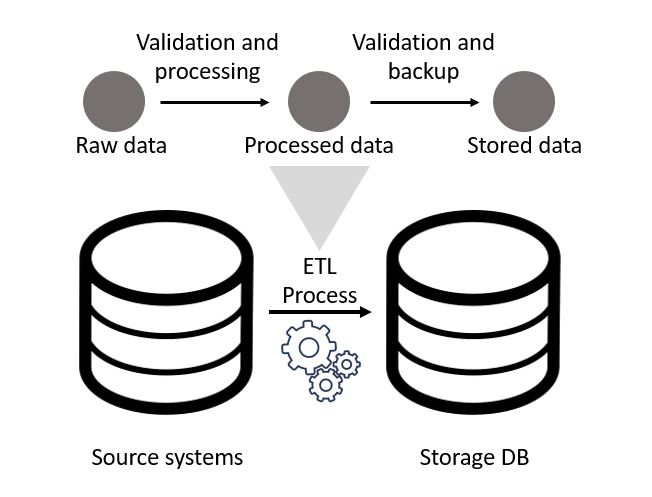
\includegraphics[width=0.5\textwidth,height=0.5\textheight]{/img/GE-setup/pipeline_testing.jpg}

To summarise the library, GE works in addition to unit / integration
testing by profiling data sources in order to build a set of
``expectations'' around each column based on the type, which can then be
pruned / added to by the user. For example, on the dataframe shown below
we have and ID column that you may expect to never be NULL, an Animal
column that should always be a string and a cost that should always be a
float.

\begin{Shaded}
\begin{Highlighting}[]

\ImportTok{import}\NormalTok{ pandas }\ImportTok{as}\NormalTok{ pd}

\NormalTok{df }\OperatorTok{=}\NormalTok{ pd.DataFrame(}\BuiltInTok{zip}\NormalTok{([}\DecValTok{1}\NormalTok{, }\DecValTok{2}\NormalTok{, }\DecValTok{3}\NormalTok{, }\DecValTok{4}\NormalTok{, }\DecValTok{5}\NormalTok{], [}\StringTok{"Cat"}\NormalTok{, }\StringTok{"Dog"}\NormalTok{, }\StringTok{"Cat"}\NormalTok{, }\StringTok{"Rabbit"}\NormalTok{, }\StringTok{"Dog"}\NormalTok{], [}\DecValTok{70}\NormalTok{, }\FloatTok{65.00}\NormalTok{, }\FloatTok{120.50}\NormalTok{, }\FloatTok{20.75}\NormalTok{, }\FloatTok{1000.00}\NormalTok{]), columns }\OperatorTok{=}\NormalTok{ [}\StringTok{"ID"}\NormalTok{, }\StringTok{"Animal"}\NormalTok{, }\StringTok{"Treatment_Cost"}\NormalTok{])}

\BuiltInTok{print}\NormalTok{(df)}
\end{Highlighting}
\end{Shaded}

\begin{verbatim}
##    ID  Animal  Treatment_Cost
## 0   1     Cat           70.00
## 1   2     Dog           65.00
## 2   3     Cat          120.50
## 3   4  Rabbit           20.75
## 4   5     Dog         1000.00
\end{verbatim}

The diagram below gives an example flow of a GE pipeline, involving
initial profiling of data, adaption of the produced expectations,
continual validation of new data against said expectations and updates
provided in auto produced html which can be deployed as a static
website, giving a very quick data quality dashboard, an example of which
from the packages docs is shown below.

\hypertarget{getting-started-with-ge-on-databricks}{%
\subsection{Getting started with GE on
databricks}\label{getting-started-with-ge-on-databricks}}

As eluded to in the title of this post, I've been utilising GE on the
well known Spark platform Databricks, as we've been using this platform
with a number of clients in order to do distributed computation of large
datasets. However, whilst this post is based around Spark, GE can work
with other datatypes such as CSVs (via Pandas Dataframes) and Relational
Databases (via SQL Alchemy), as shown in their docs here
(\url{https://docs.greatexpectations.io/en/latest/getting_started/cli_init.html}).

So, in order to start using GE in DataBricks you must first follow the
initialisation instructions on your local machine, after downloading
from PyPy both locally and on your Databricks cluster. These
instructions are provided here
(\url{https://docs.greatexpectations.io/en/latest/getting_started/cli_init.html}),
however at the add datasource stage choose option 4, which will lead to
set up completing with no allocated datasource. The next step is to go
into the great\_expectations.yaml file in order to set up the required
datasource, by adding in the lines shown below.

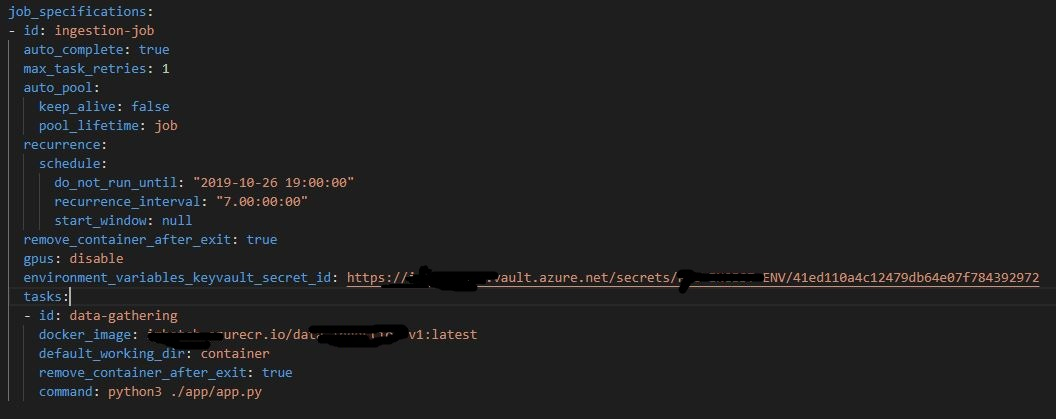
\includegraphics[width=1\textwidth,height=1\textheight]{/img/GE-setup/yaml.jpg}

Once this is saved you can copy the local files over into the DataBricks
File System (DBFS), using the DataBricks CLI, as shown below and
documented here
(\url{https://docs.databricks.com/dev-tools/cli/dbfs-cli.html}). This
involves first making a directory in the DBFS and then copying over the
files.

\begin{Shaded}
\begin{Highlighting}[]
\NormalTok{dbfs mkdirs your_ge_dir}

\CommentTok{#Note this \textbackslash{} is for Windows, change to / for linux}
\NormalTok{dbfs cp }\OperatorTok{-}\NormalTok{r .\textbackslash{}your_local_folder dbfs}\OperatorTok{:}\ErrorTok{/}\NormalTok{your_ge_dir}
\end{Highlighting}
\end{Shaded}

Once this is done you can check the files have copied by opening a
notebook, and using the \%fs cell magic to check the contents of your
dbfs, using the below code.

\begin{Shaded}
\begin{Highlighting}[]
\NormalTok{%fs}

\NormalTok{ls your_new_dir}\OperatorTok{/}
\end{Highlighting}
\end{Shaded}

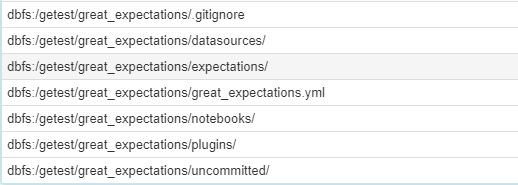
\includegraphics[width=0.5\textwidth,height=0.5\textheight]{/img/GE-setup/ge_dbfs.jpg}

Now that you have the initilisation set up and the library on your
cluster you can set your GE context (which tells the profiler what kind
of data to expect) and set your initial expectations, which I'll
document in two different ways, manual profiling and full profiling.

\hypertarget{setting-your-expectations---setup}{%
\subsubsection{Setting your expectations -
Setup}\label{setting-your-expectations---setup}}

To do either of the above mentioned methods there is a standard set up,
which is shown below. This just sets up your data context and builds a
list of your data assets in a specific database, and then adds a list
with paths of where to store the expectations.

\begin{Shaded}
\begin{Highlighting}[]
\NormalTok{import great_expectations as ge}

\NormalTok{DATABASE =}\StringTok{ "database"}

\NormalTok{context =}\StringTok{ }\KeywordTok{ge.data_context.DataContext}\NormalTok{(}\StringTok{"/dbfs/your_ge_dir/great_expectations/"}\NormalTok{)}

\NormalTok{generator =}\StringTok{ }\KeywordTok{ge.datasource.generator.databricks_generator.DatabricksTableGenerator}\NormalTok{(}\DataTypeTok{name =} \StringTok{'default'}\NormalTok{, }\DataTypeTok{datasource =}\NormalTok{ None, }\DataTypeTok{database =}\NormalTok{ DATABASE)}

\NormalTok{data_assets =}\StringTok{ }\KeywordTok{generator.get_available_data_asset_names}\NormalTok{()}

\NormalTok{data_assets_paths =}\StringTok{ }\NormalTok{[}\StringTok{"spark/passthrough/"} \OperatorTok{+}\StringTok{ }\NormalTok{i }\ControlFlowTok{for}\NormalTok{ i }\ControlFlowTok{in}\NormalTok{ data_assets]}
\end{Highlighting}
\end{Shaded}

\hypertarget{method-1-manual-profiling}{%
\subsubsection{Method 1: Manual
Profiling}\label{method-1-manual-profiling}}

The first step to manual profiling is to set up the batch kwargs for the
dataset in question, which allows GE to know what batch of data is being
profiled, and the asset path in order to produce an empty expectations
file.

\begin{Shaded}
\begin{Highlighting}[]
\NormalTok{batch_kwargs =}\StringTok{ }\NormalTok{\{}\StringTok{"dataset"} \OperatorTok{:}\StringTok{ }\KeywordTok{spark.table}\NormalTok{(f}\StringTok{"\{database\}.\{data_assets[0]\}"}\NormalTok{)\}}

\NormalTok{data_asset_name =}\StringTok{ }\NormalTok{data_assets_paths[}\DecValTok{0}\NormalTok{]}

\KeywordTok{context.create_expectation_suite}\NormalTok{(data_asset_name, }\StringTok{"Test"}\NormalTok{)}

\NormalTok{batch =}\StringTok{ }\KeywordTok{context.get_batch}\NormalTok{(data_asset_name, }\StringTok{"Test"}\NormalTok{, batch_kwargs)}
\end{Highlighting}
\end{Shaded}

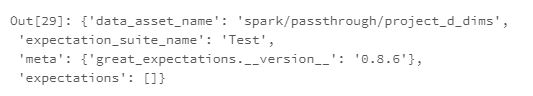
\includegraphics[width=1\textwidth,height=1\textheight]{/img/GE-setup/empty_expectation.jpg}

Once you have your empty file you can manually add in the relevant
expectations for the desired columns, and profile the batch of data via
the validation operator, save out the new expectation suite (in this
scenario also saving any failed expectations) and build the static html
for the data quality docs, an example of which is shown below.

\begin{Shaded}
\begin{Highlighting}[]
\KeywordTok{batch.expect_column_values_to_not_be_null}\NormalTok{(}\StringTok{"PROJECT_ID"}\NormalTok{)}
\KeywordTok{batch.expect_column_values_to_be_in_set}\NormalTok{(}\StringTok{"DELIVERY_GROUP_LATEST"}\NormalTok{, }\KeywordTok{set}\NormalTok{([}\StringTok{'IP Legacy'}\NormalTok{, }\StringTok{'IP AM SP&C'}\NormalTok{]))}
\KeywordTok{batch.expect_column_distinct_values_to_be_in_set}\NormalTok{(}\StringTok{"DELIVERY_GROUP_LATEST"}\NormalTok{, }\KeywordTok{set}\NormalTok{([}\StringTok{'IP Legacy'}\NormalTok{, }\StringTok{'IP AM SP&C'}\NormalTok{]))}

\KeywordTok{context.run_validation_operator}\NormalTok{(}\StringTok{"action_list_operator"}\NormalTok{, [batch])}

\KeywordTok{batch.save_expectation_suite}\NormalTok{(}\DataTypeTok{discard_failed_expectations =}\NormalTok{ False)}

\KeywordTok{context.build_data_docs}\NormalTok{()}
\end{Highlighting}
\end{Shaded}

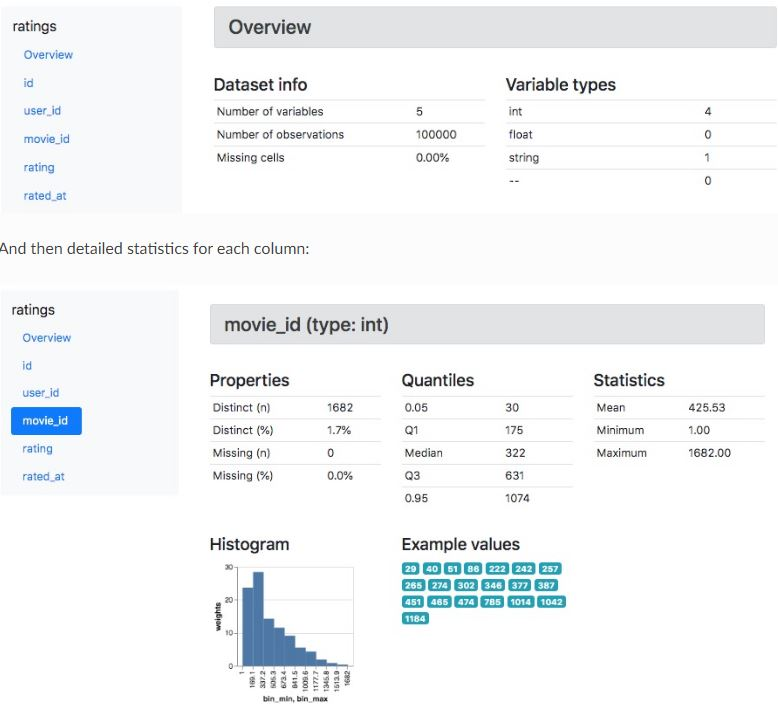
\includegraphics[width=0.5\textwidth,height=0.5\textheight]{/img/GE-setup/data_docs.jpg}

\hypertarget{method-2-full-profiling}{%
\subsubsection{Method 2: Full Profiling}\label{method-2-full-profiling}}

As opposed to manual profiling, full profiling utilises the inbuilt data
profiler that is packaged with GE in order to build a full expectation
suite based on the column types, and then validate the data against all
of these expectations. A workflow for such a method might be to profile
all the tables within a database, maintain these expectations and then
validate any updates from the raw data that is appended to these tables.
This example is what is shown below, which utilises a couple of custom
functions which can be applied to each table within the data asset list
created during set up.

\begin{Shaded}
\begin{Highlighting}[]
\CommentTok{# First build the functions to produce the expectations for the database and also}
\CommentTok{# to run the validations }

\NormalTok{def }\KeywordTok{create_initial_expectations_suite}\NormalTok{(database, asset_name, context, asset_path)}\OperatorTok{:}
\StringTok{  }
\StringTok{  }\NormalTok{data =}\StringTok{ }\KeywordTok{spark.table}\NormalTok{(database }\OperatorTok{+}\StringTok{ "."} \OperatorTok{+}\StringTok{ }\NormalTok{asset_name)}
  
\NormalTok{  batch_kwargs =}\StringTok{ }\NormalTok{\{}\StringTok{"dataset"} \OperatorTok{:}\StringTok{ }\NormalTok{data\}}
  
  \KeywordTok{context.create_expectation_suite}\NormalTok{(asset_path, f}\StringTok{"\{asset_name\}_\{database\}_expectations"}\NormalTok{, }\DataTypeTok{overwrite_existing =}\NormalTok{ True)}
  
\NormalTok{  batch =}\StringTok{ }\KeywordTok{context.get_batch}\NormalTok{(asset_path, f}\StringTok{"\{asset_name\}_\{database\}_expectations"}\NormalTok{, batch_kwargs)}
  
\NormalTok{  expectation_suite, validation_result =}\StringTok{ }\KeywordTok{BasicDatasetProfiler.profile}\NormalTok{(batch)}
  
  \KeywordTok{context.save_expectation_suite}\NormalTok{(expectation_suite)}
  
  
\NormalTok{def }\KeywordTok{run_validations}\NormalTok{(database, asset_name, context, asset_path)}\OperatorTok{:}
\StringTok{  }
\StringTok{  }\NormalTok{data =}\StringTok{ }\KeywordTok{spark.table}\NormalTok{(database }\OperatorTok{+}\StringTok{ "."} \OperatorTok{+}\StringTok{ }\NormalTok{asset_name)}
  
\NormalTok{  batch_kwargs =}\StringTok{ }\NormalTok{\{}\StringTok{"dataset"} \OperatorTok{:}\StringTok{ }\NormalTok{data\}}
  
\NormalTok{  batch =}\StringTok{ }\KeywordTok{context.get_batch}\NormalTok{(asset_path, f}\StringTok{"\{asset_name\}_\{database\}_expectations"}\NormalTok{, batch_kwargs)}
  
\NormalTok{  val_run =}\StringTok{ }\KeywordTok{batch.validate}\NormalTok{()}
  
\NormalTok{  with }\KeywordTok{open}\NormalTok{(}\StringTok{"/dbfs/getest/great_expectations/expectations/spark/passthrough/dss_parameter/validation.txt"}\NormalTok{, }\StringTok{'w'}\NormalTok{) as f}\OperatorTok{:}
\StringTok{    }\KeywordTok{json.dump}\NormalTok{(val_run, f)}
  
  \KeywordTok{context.run_validation_operator}\NormalTok{(}\StringTok{"action_list_operator"}\NormalTok{, [batch])  }
  
  \KeywordTok{context.build_data_docs}\NormalTok{()}
\end{Highlighting}
\end{Shaded}

\begin{Shaded}
\begin{Highlighting}[]
\CommentTok{# Import the profiler, create the expectations and then validate, storing the }
\CommentTok{# results of the validation and updating the data docs}

\NormalTok{from great_expectations.profile.basic_dataset_profiler import BasicDatasetProfiler}


\ControlFlowTok{for}\NormalTok{ i, j }\ControlFlowTok{in} \KeywordTok{zip}\NormalTok{(data_assets, data_assets_paths)}\OperatorTok{:}
\StringTok{  }\KeywordTok{create_initial_expectations_suite}\NormalTok{(DATABASE, i, context, j)}


\ControlFlowTok{for}\NormalTok{ i, j }\ControlFlowTok{in} \KeywordTok{zip}\NormalTok{()}\OperatorTok{:}
\StringTok{  }\KeywordTok{run_validations}\NormalTok{(DATABASE, i, context, j)}
\end{Highlighting}
\end{Shaded}

The first function should produce an expectations file for each table,
which can then be validated against to build a new data docs page.
Examples of the json outputs from both functions are shown below.

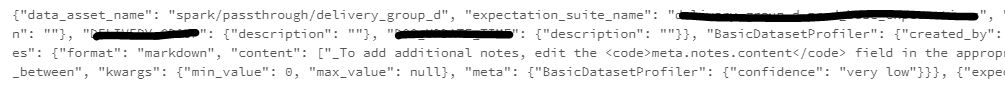
\includegraphics[width=1\textwidth,height=1\textheight]{/img/GE-setup/empty_profile.jpg}

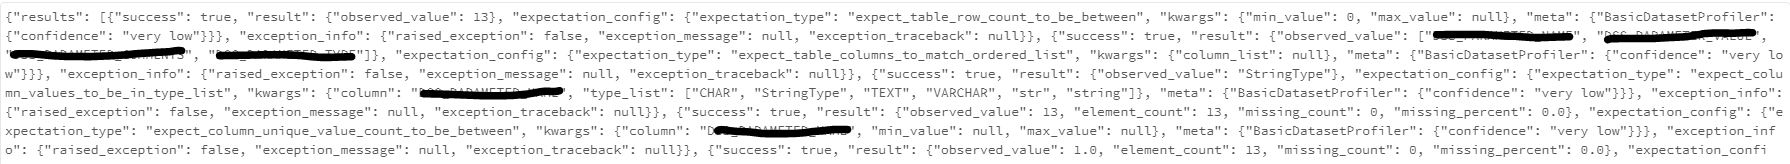
\includegraphics[width=1\textwidth,height=1\textheight]{/img/GE-setup/full_profile.jpg}

\hypertarget{wrap-up}{%
\subsection{Wrap up}\label{wrap-up}}

So, hopefully this post has shown you a potential new way to more simply
test the quality of what's moving within your data pipeline, rather than
just the functions that are make it up! In addition to the enhanced
testing that GE provides, I believe that the incorporation of the static
Data Docs data quality pages could be a real help to organisations
looking to quickly understand the quality of their data!


\end{document}
